\documentclass[mathserif, handout]{beamer}
% ======================================================================
% General LaTeX Setup for Beamer (Reusable Preamble)
% Author: Chandra Gummaluru
% ======================================================================

\documentclass[mathserif, handout]{beamer}
\setbeamertemplate{frametitle}{}

% ------------------------------------------------------------
% basic packages
% ------------------------------------------------------------
\usepackage{url}
\usepackage{ifthen}
\usepackage{enumerate}
\usepackage[font=small]{caption}
\usepackage{subcaption}
\usepackage{moresize}
\usepackage[outline]{contour}
\usepackage{transparent}
\usepackage{worldflags}
\usepackage{bm}
\usepackage{graphbox}
\usepackage{mathtools}
\usepackage{multirow}
\usepackage{fontawesome5}
\usepackage{pifont}
\usepackage{array}
\usepackage{comment}

% ------------------------------------------------------------
% math
% ------------------------------------------------------------
\DeclarePairedDelimiter{\floor}{\lfloor}{\rfloor}
\DeclarePairedDelimiter{\ceil}{\lceil}{\rceil}

% ------------------------------------------------------------
% colors
% ------------------------------------------------------------
\definecolor{hl}{RGB}{248,196,69}
\definecolor{myred}{HTML}{ED5565}
\definecolor{myorange}{HTML}{FC6E51}
\definecolor{myyellow}{HTML}{FFCE54}
\definecolor{mycyan}{HTML}{4FC1E9}
\definecolor{myblue}{HTML}{5D9CEC}

\newcommand{\graytext}[1]{\footnotesize\color{gray}#1\normalsize\color{black}}

% ------------------------------------------------------------
% symbols
% ------------------------------------------------------------
\newcommand{\cmark}{\ding{51}}
\newcommand{\xmark}{\ding{55}}

% ------------------------------------------------------------
% highlighting
% ------------------------------------------------------------
\newcommand{\reducedstrut}{\vrule width 0pt height .9\ht\strutbox depth .9\dp\strutbox\relax}
\newcommand{\highlight}[1]{%
  \begingroup\setlength{\fboxsep}{0pt}\colorbox{hl}{\reducedstrut$\displaystyle #1$\/}\endgroup}
\newcommand{\highlightc}[2]{%
  \begingroup\setlength{\fboxsep}{0pt}\colorbox{#1}{\reducedstrut$\displaystyle #2$\/}\endgroup}

% ------------------------------------------------------------
% environments (boxes)
% ------------------------------------------------------------
\usepackage{tcolorbox}
\tcbuselibrary{skins}

\newtcolorbox{thmbox}[1][]{colback=gray!30!white!20, colframe=black, fonttitle=\bfseries, title=#1, boxrule=0.5pt}

% 1) Bottom open (draw top + sides only)
\newtcolorbox{thmboxtop}[1][]{
    enhanced,
    frame hidden,
    colback=gray!30!white!20,
    borderline north={0.5pt}{0pt}{black}, % top
    borderline west={0.5pt}{0pt}{black},  % left
    borderline east={0.5pt}{0pt}{black}   % right
}

% 2) Top open (draw bottom + sides only)
\newtcolorbox{thmboxbot}[1][]{
    enhanced,
    frame hidden,
    colback=gray!30!white!20,
    borderline south={0.5pt}{0pt}{black}, % bottom
    borderline west={0.5pt}{0pt}{black},  % left
    borderline east={0.5pt}{0pt}{black}   % right
}

% 3) Side only (draw only left and right)
\newtcolorbox{thmboxside}[1][]{
    enhanced,
    frame hidden,
    colback=gray!30!white!20,
    borderline west={0.5pt}{0pt}{black},  % left
    borderline east={0.5pt}{0pt}{black}   % right
}

\newtcolorbox{defboxtop}[1][]{
    enhanced,
    colback=gray!30!white!20,
    frame hidden,
    overlay={
        % Draw top + sides with rounded corners
        \draw[line width=0.5pt, black, rounded corners=3mm]
            (frame.south west) -- (frame.north west) -- (frame.north east) -- (frame.south east);
    },
    #1
}

\newtcolorbox{defboxbot}[1][]{
    enhanced,
    colback=gray!30!white!20,
    frame hidden,
    overlay={
        % Draw top + sides with rounded corners
        \draw[line width=0.5pt, black, rounded corners=3mm]
            (frame.north west) -- (frame.south west) -- (frame.south east) -- (frame.north east);
    },
    #1
}

\newtcolorbox{defboxside}[1][]{
    enhanced,
    frame hidden,
    colback=gray!30!white!20,
    borderline west={0.5pt}{0pt}{black},  % left
    borderline east={0.5pt}{0pt}{black}   % right
}

\newtcolorbox{proofbox}[1][]{colback=gray!20!white!20, colframe=grey, fonttitle=\bfseries, title=#1, boxrule=0.5pt, colbacktitle=white, enhanced jigsaw, sharp corners}

% ------------------------------------------------------------
% code listings
% ------------------------------------------------------------
\usepackage{listings}
\lstdefinestyle{mypython}{
  language=Python,
  deletekeywords=[2]{open, next, from, chr, str, int},
  morekeywords=[3]{List, Graph, Tree, Dict, Set, UnionFind, Ordict, Trie, Queue},
  morekeywords=[4]{ListNode, Vertex, Edge, Path, TreeNode, DictNode, UnifNode, OrdictNode, TrieNode, QueueNode},
  morekeywords=[5]{True, False, Boolean, String, Integer, Key, Function, KeyedObject, Object, Array, Tuple, Optional, None},
  keywordstyle=\color{mycyan}\bfseries,
  keywordstyle=[3]\color{myblue}\bfseries,
keywordstyle=[4]\color{myblue}\bfseries,
keywordstyle=[5]\color{mycyan}\bfseries,
  stringstyle=\color{orange},
  commentstyle=\color{gray}\itshape,
  basicstyle=\ttfamily\footnotesize,
  numbers=left,
  numberstyle=\tiny\color{gray},
  stepnumber=1,
  numbersep=5pt,
  xleftmargin=15pt,
  frame=none,
  showstringspaces=false,
  breaklines=true,
  breakatwhitespace=true,
  tabsize=4,
  columns=flexible
}


% ------------------------------------------------------------
% algorithms
% ------------------------------------------------------------
\usepackage{algorithm}
\usepackage[endLComment=~]{algpseudocodex}
\makeatletter
\algrenewcommand\ALG@beginalgorithmic{\footnotesize}
\makeatother

% ------------------------------------------------------------
% optimization environments
% ------------------------------------------------------------
\usepackage[nocomma]{optidef}

% ------------------------------------------------------------
% pgfplots and pie charts
% ------------------------------------------------------------
\usepackage{pgfplots}
\usepackage{pgf-pie}
\pgfplotsset{compat=1.7}

% ------------------------------------------------------------
% tikz
% ------------------------------------------------------------
\usepackage{tikz}
\usetikzlibrary{
  angles, quotes, positioning, fit, backgrounds, shapes.geometric, intersections,
  calc, shapes, mindmap, decorations.text, arrows, arrows.meta,
  automata, chains, decorations.pathreplacing, calligraphy,
  decorations.markings, shapes.misc, decorations.pathmorphing
}
\tikzset{
  invisible/.style={opacity=0},
  visible on/.style={alt=#1{}{invisible}},
  alt/.code args={<#1>#2#3}{\alt<#1>{\pgfprioritysalso{#2}}{\pgfprioritysalso{#3}}}
}

\newcommand{\multiedge}[5][]{
\pgfmathsetmacro{\N}{#4}
\pgfmathsetmacro{\mid}{(\N-1)/2}
\foreach \i in {0,...,\numexpr#4-1\relax} {

\pgfmathsetmacro{\k}{\i-\mid}
\draw[#1] ($ (#2) + \k*#5*($(#2)!1!90:(#3)$) $) -- ($ (#3) + \k*#5*($(#2)!1!90:(#3)$) $); 

}
\draw[#1,  -{>[scale=1]}]
  ($(#2)!0.54!(#3)$) -- ($(#2)!0.55!(#3)$);
}

% ------------------------------------------------------------
% bibliography
% ------------------------------------------------------------
\usepackage[style=ieee]{biblatex}
\setbeamertemplate{bibliography item}{\insertbiblabel}
\setbeamertemplate{background canvas}{
  \begin{tikzpicture}[remember picture,overlay]
    \node[opacity=0.0075]
      at (current page.center)
      {
\includegraphics[width=0.8\paperwidth]{images/signature.pdf}};
  \end{tikzpicture}
}

% ------------------------------------------------------------
% beamer theme and settings
% ------------------------------------------------------------
\usetheme{Boadilla}
\usecolortheme{seagull}
\beamertemplatenavigationsymbolsempty
\setbeamertemplate{enumerate item}{(\arabic{enumi})}
\setbeamertemplate{enumerate subitem}{(\alph{enumii})}
\setbeamertemplate{enumerate subsubitem}{(\roman{enumiii})}
\setbeamertemplate{itemize item}[circle]
\setbeamertemplate{itemize subitem}{\circ}
\setbeamertemplate{itemize subsubitem}{-}
\setbeamercolor{item}{fg=black!40}
\setbeamercovered{transparent=10}

% ===========================
% Premade TikZ Figure Commands
% ===========================

% images w/ labels
% inside tikz as a node
\NewDocumentCommand{\labeledimgnodetikz}{O{} m m m m m m}{%
	\begin{scope}[transparency group, #1]
		\node[
			draw,
			circle,
			inner sep=0,
			outer sep=0,
			minimum size=10mm,
			#1
		] (#5) at (#3,#4)
		{\includegraphics[scale=#7]{#6}};
		\node[
			rectangle,
			draw=black,
			thick,
			fill=black!55,
			rounded corners=0.1mm,
			inner sep=0pt,
			outer sep=0pt,
			minimum size=2.8mm,
			minimum width=3.5mm
		] at (#3,#4-0.1) {};
		\node[outer sep=0, inner sep=0, white] at (#3,#4-0.1) {\footnotesize #2};
	\end{scope}
}

% inside tikz isolated

% outside tikz
\NewDocumentCommand{\labelednode}{m}{%
	\begin{tikzpicture}[baseline={(0,-1mm)}]
		\node[
			rectangle,
			thick,
			draw=black,
			fill=black!55,
			rounded corners=0.1mm,
			inner sep=0pt,
			outer sep=0pt,
			minimum size=2.8mm,
			minimum width=3.5mm
		] at (0,0) {};
		\node[outer sep=0, inner sep=0, white, minimum size=2.8mm, minimum width=3.5mm] at (0,0) {\footnotesize #1};
	\end{tikzpicture}
}

% images only
% inside tikz as a node
\NewDocumentCommand{\imgnodetikz}{O{} m m m m m m}{%
	\begin{scope}[transparency group, #1]
		\node[
			draw,
			circle,
			inner sep=0,
			outer sep=0,
			minimum size=10mm,
			#1
		] (#5) at (#3,#4)
		{\includegraphics[scale=#7]{#6}};
		\node[
			rectangle,
			draw,
			thick,
			fill=black!55,
			rounded corners=0.1mm,
			inner sep=0pt,
			outer sep=0pt,
			minimum size=2.8mm,
			minimum width=3.5mm,
			opacity=0
		] at (0,0) {};
		\node[outer sep=0, inner sep=0, white, opacity=0] at (0,0) {\footnotesize #2};
	\end{scope}
}

% inside tikz isolated
\NewDocumentCommand{\imgtikz}{O{} mm}{%
	\begin{scope}[transparency group, #1]
		\node[
			inner sep=0,
			outer sep=0
		] (#5) at (#3,#4)
		{\includegraphics[scale=#3]{#2}};
	\end{scope}
}


% outside tikz
\NewDocumentCommand{\imgnode}{mm}{%
	\begin{tikzpicture}[baseline={(0,-1mm)}]
        \node[
            inner sep=0,
            outer sep=0,
            draw opacity=0,
        ] at (0,0)
        {\includegraphics[scale=#2]{#1}};
    \end{tikzpicture}
}

% outside tikz (inline)
\newcommand{\imgnodetext}[2]{%
	\hspace{-0.5mm}%
	\raisebox{-0.26\height}{%
		\includegraphics[scale=#2]{#1}%
	}%
	\hspace{-0.5mm}%
}


% labels only
% inside tikz as a node
\NewDocumentCommand{\labeltikz}{m}{%
	\node[
		rectangle,
		thick,
		draw=black,
		fill=black!55,
		rounded corners=0.1mm,
		inner sep=0pt,
		outer sep=0pt,
		minimum size=2.8mm,
		minimum width=3.5mm
	] at (0,0) {};
	\node[outer sep=0, inner sep=0, white, draw opacity=0] at (0,0) {\footnotesize #1};
}

% inside tikz isolated

% outside tikz

% === define custom pgfkeys ===
\pgfkeys{
	/devicenode/.is family, /devicenode,
	outline thickness/.initial=thick,
	outline color/.initial=black
}

\NewDocumentCommand{\qpacket}{m}{%
	\begin{tikzpicture}[baseline=(current bounding box.center)]
		\node at (0.5,0.4) {\includegraphics[scale=0.1]{#1}};
	\end{tikzpicture}%
}

\NewDocumentCommand{\bpacketid}{mmm}{%
	\begin{tikzpicture}[baseline=(current bounding box.center)]
		\begin{scope}[shift={(0.85,0.7)}]
			\draw[thick, draw=black, fill=#1, rounded corners=1pt] (0.01,0.05) rectangle node[white, text width=1cm, align=center] {\color{#3}\footnotesize #2} (-0.71,-0.625);
		\end{scope}
	\end{tikzpicture}%
}

\NewDocumentCommand{\packetid}{mmmm}{%
	\begin{tikzpicture}[baseline=(current bounding box.center)]
		\begin{scope}[shift={(0.85,0.7)}]
			\draw[thick, draw=black, fill=#2, rounded corners=1pt] (0.01,0.05) rectangle node[white, text width=1cm, align=center] {\color{#4}\footnotesize #3} (-0.71,-0.625);
			\node[
				star,
				star points=30,
				star point ratio=0,
				scale=1.5,
				draw=black,
				thick,
				fill=white,
				rounded corners=0.1mm,
				inner sep=0pt,
				minimum size=2.8mm
			] at (0,0) {};
			\node at (0,0) {\footnotesize #1};
		\end{scope}
	\end{tikzpicture}%
}

\tikzset{
	dictnode/.pic={
			\draw[thick, fill=#1, line join=]
			(-0.75,-0.5) --
			(-0.75,0.5)  --
			(0.75,0.5) --
			(0.75,-0.5) --
			cycle --
			(-0.75, 0.75) --
			(0.75, 0.75) --
			(0.75, -0.5) --
			cycle;
		}
}

\tikzset{
	queuenode/.pic={
			\draw[thick, fill=#1, line join=round]
			(-0.85,-0.5) --
			(-0.85,0.5)  --
			(0.65,0.5) --
			(0.75,0) --
			(0.65,-0.5) --
			cycle;
		}
}

\tikzset{
	queuenodetail/.pic={
			\draw[thick, fill=#1, line join=round]
			(-0.75,-0.5) --
			(-0.75,0.5)  --
			(0.65,0.5) --
			(0.75,0) --
			(0.65,-0.5) --
			cycle;
		}
}

\tikzset{
	listnode/.style={
			shape=rectangle,
			rounded corners,
			thick,
			minimum height=10mm,
			minimum width=15mm,
			inner sep=0pt
		}
}

\tikzset{
	arraynode/.style={
			shape=rectangle,
			thick,
			minimum height=10mm,
			minimum width=15mm,
			inner sep=0pt
		}
}

\tikzset{
	graphnode/.style={
			shape=circle,
			thick,
			minimum size=5mm,
			inner sep=0pt
		}
}

\tikzset{
	defaultnode/.style={
			transform shape,
			circle,
			draw=black,
			thick,
			fill=white,
			minimum size=10mm,
			inner sep=0pt
		},
	newnode/.style={
			transform shape,
			defaultnode,
			draw=myyellow,
			fill=myyellow!60,
			very thick
		},
	newnodelight/.style={
			transform shape,
			defaultnode,
			draw=myyellow,
			fill=myyellow!30,
			very thick
		},
	deletenode/.style={
			defaultnode,
			draw=gray,
			dashed,
			fill=lightgray,
			text=gray,
			very thick
		},
	nooutlinenode/.style={
			defaultnode,
			draw=none,
            draw opacity=0,
			text=black,
			very thick
		},
    nofillnode/.style={
			defaultnode,
			fill=none,
            text=black,
			very thick
		}
}
\tikzset{
	faded/.style={opacity=0.5, text opacity=0.5, transparency group}
}
\tikzset{
	smallgraytext/.style={font=\footnotesize\color{gray}}
}
\tikzset{
	graytext/.style={font=\normalsize\color{gray}}
}
\tikzset{
  squigglearrow/.style={
    very thick,
    lightgray,
    decorate,
    decoration={
      snake,
      amplitude=1.75pt,
      segment length=8pt
    }
  }
}



% title
\title{Queues}
\subtitle{Algorithms and Data Structures}
\author[C. Gummaluru]{Chandra Gummaluru}
\titlegraphic{
\includegraphics[width=0.15\linewidth]{images/signature.pdf}}
\institute[]{\url{chandra-gummaluru.github.io} }
\date[Algorithms and Data Structures]{}

\begin{document}

\begin{frame}
   \maketitle
\end{frame}

\begin{frame}{Motivation}
\begin{center}
    \Large \highlight{\textbf{motivation}}
\end{center}
\end{frame}

\begin{frame}
A communication tower receives packets of different types and sizes, arriving at various times from multiple flows.
\begin{figure}
    \centering
    \begin{tikzpicture}
        \node (s) at (3,0) {
\includegraphics[scale=0.2]{images/radio_tower.png}};
        \node[below = 0mm of s, align=center, text width = 1cm] {\color{gray}\footnotesize router};

        
        \node (v) at (-3,1.5) {
\includegraphics[scale=0.1]{images/video_icon.png}};
        \node[left = 0mm of v, align=right, text width = 1cm] {\color{gray}\footnotesize video\\[-1mm]packet};
        
        \node (m) at (-3,0.5) {
\includegraphics[scale=0.1]{images/music_icon.png}};
        \node[left = 0mm of m, align=right, text width = 1cm] {\color{gray}\footnotesize audio\\[-1mm]packet};
        
        \node (p) at (-3,-0.5) {
\includegraphics[scale=0.1]{images/picture_icon.png}};
        \node[left = 0mm of p, align=right, text width = 1cm] {\color{gray}\footnotesize picture\\[-1mm]packet};
        
        \node (t) at (-3,-1.5) {
\includegraphics[scale=0.1]{images/text_icon.png}};
        \node[left = 0mm of t, align=right, text width = 1cm] {\color{gray}\footnotesize text\\[-1mm]packet};

        \draw[very thick, ->] (v) edge (s);
        \draw[very thick, ->] (m) edge (s);
        \draw[very thick, ->] (p) edge (s);
        \draw[very thick, ->] (t) edge (s);
    \end{tikzpicture}
\end{figure}
\vspace{-2mm}
Some packets (e.g., video/audio packets) are more time-sensitive than others, but the tower can only send one packet at a time.
\end{frame}

\begin{frame}
For simplicity, we assume that: \\[2mm]
    \begin{itemize}
        \item all packets of a given type take the same amount of time to transmit:\\[2mm]
        \begin{center}
                    \begin{tikzpicture}
        \node (A1) at (4,0) {
\includegraphics[scale=0.1]{images/music_icon.png}} node[below=0cm of A1, text width = 2cm, align=center] {\color{gray}\footnotesize 6 ts};
        \node (P1) at (2,0) {
\includegraphics[scale=0.1]{images/picture_icon.png}} node[below=0cm of P1, text width = 2cm, align=center] {\color{gray}\footnotesize 4 ts};

        \node (T1) at (0,0) {
\includegraphics[scale=0.1]{images/text_icon.png}} node[below=0cm of T1, text width = 2cm, align=center] {\color{gray}\footnotesize 2 ts};
        \node (V1) at (6,0) {
\includegraphics[scale=0.1]{images/video_icon.png}} node[below=0cm of V1, text width = 2cm, align=center] {\color{gray}\footnotesize 8 ts};
    \end{tikzpicture}
            
        \end{center}
        \item each flow represents packets of a given type
        \item no two packets arrive at the same time-step
        \item each packet contains all relevant information for routing purposes\\[2mm]
    \end{itemize}
    
\end{frame}

\begin{frame}
Suppose the tower receives the following packets:
\begin{center}
    \begin{tikzpicture}
    
        \node (V1) at (0,0) {\qpacket{images/music_icon.png}} node[below=-2mm of V1, text width = 2cm, align=center] {\color{gray}\footnotesize ts 0};
        
        \node (A1) at (1.75,0) {\qpacket{images/picture_icon.png}} node[below=-2mm of A1, text width = 2cm, align=center] {\color{gray}\footnotesize ts 2};
        \node (P1) at (3.5,0) {\qpacket{images/text_icon.png}} node[below=-2mm of P1, text width = 2cm, align=center] {\color{gray}\footnotesize ts 3};
        
        \node (T1) at (5.25,0) {\qpacket{images/text_icon.png}} node[below=-2mm of T1, text width = 2cm, align=center] {\color{gray}\footnotesize ts 4};
        \node (T2) at (7,0) {\qpacket{images/music_icon.png}} node[below=-2mm of T2, text width = 2cm, align=center] {\color{gray}\footnotesize ts 5};
        \node (A2) at (8.75,0) {\qpacket{images/video_icon.png}} node[below=-2mm of A2, text width = 2cm, align=center] {\color{gray}\footnotesize ts 6};

        \draw[very thick] (0.25,-1.4) edge[bend right, <->] node[midway, below, text width=4cm, align=center] {\color{gray}\footnotesize packets from \\[-1mm] an audio flow} (6.75,-1.4);
    \end{tikzpicture}
\end{center}
    
\end{frame}

\begin{frame}
Without any prioritization, packets can be stored in a queue:
\begin{center}
    \begin{tikzpicture}

\coordinate (mA) at (-1.5,0);
\coordinate (mB) at (0,0);
\coordinate (mC) at (1.5,0);
\coordinate (mD) at (3,0);
\coordinate (mE) at (4.5,0);
\coordinate (mF) at (6,0);
\coordinate (mG) at (7.5,0);

\pic at (mG) {queuenode={lightgray!10}};
\pic at (mF) {queuenode={lightgray!10}};
\pic at (mE) {queuenode={lightgray!10}};
\pic at (mD) {queuenode={lightgray!10}};
\pic at (mC) {queuenode={lightgray!10}};
\pic at (mB) {queuenode={lightgray!10}};
\pic at (mA) {queuenodetail={lightgray!10}};

\node (p1) at (0,0) {\footnotesize\hspace{1.5mm}6,\hspace{-0.25mm}\raisebox{1mm}{\qpacket{images/video_icon.png}}};
\node (p2) at (1.5,0) {\footnotesize\hspace{1.5mm}5,\hspace{-0.25mm}\raisebox{1mm}{\qpacket{images/music_icon.png}}};
\node (p3) at (3,0) {\footnotesize\hspace{1.5mm}4,\hspace{-0.25mm}\raisebox{1mm}{\qpacket{images/text_icon.png}}};
\node (p4) at (4.5,0) {\footnotesize\hspace{1.5mm}3,\hspace{-0.25mm}\raisebox{1mm}{\qpacket{images/text_icon.png}}};
\node (p5) at (6,0) {\footnotesize\hspace{1.5mm}2,\hspace{-0.25mm}\raisebox{1mm}{\qpacket{images/picture_icon.png}}};
\node (p6) at (7.5,0) {\footnotesize\hspace{1.5mm}0,\hspace{-0.25mm}\raisebox{1mm}{\qpacket{images/music_icon.png}}};

\end{tikzpicture}
\end{center}
    
\end{frame}

\begin{frame}
This results in a specific timing for when packets are transmitted, as shown in the graph below:
\begin{center}
\centering
    \begin{tikzpicture}
\begin{scope}[yshift=-0.25cm]  
  \draw[step=0.5cm,gray,very thin, opacity=0.3] (0,0.25) grid (10.25,3.25);
\end{scope}


  % Draw x and y axes
  \draw[thick,->] (0,0) -- (10.5,0) node[anchor=south east] {\color{gray}ts};
  \draw[thick,->] (0,0) -- (0,3.5);
  
  \draw[fill=myyellow, thick] (0,0.1) rectangle ++ (3,0.3);
  \node at (0,0.28) {\scalebox{0.55}{\qpacket{images/music_icon.png}}};
  
  \draw[thick] (1,0.75) -- (3,0.75);
  \node at (1,0.78) {\scalebox{0.55}{\qpacket{images/picture_icon.png}}};
  \draw[fill=mycyan, thick] (3,0.6) rectangle ++ (2,0.3);

  
  \draw[thick] (1.5,1.25) -- (5,1.25);
\node at (1.5,1.28) {\scalebox{0.55}{\qpacket{images/text_icon.png}}};
  \draw[fill=lightgray, thick] (5,1.1) rectangle ++ (1,0.3);
  
  \draw[thick] (2,1.75) -- (6,1.75);
  \node at (2,1.78) {\scalebox{0.55}{\qpacket{images/text_icon.png}}};
  \draw[fill=lightgray, thick] (6,1.6) rectangle ++ (1,0.3);

  \draw[thick] (2.5,2.25) -- (7,2.25);
  \node at (2.5,2.28) {\scalebox{0.55}{\qpacket{images/music_icon.png}}};
  \draw[fill=myyellow, thick] (7,2.1) rectangle ++ (3 ,0.3);
  
  \draw[thick] (3,2.75) -- (10,2.75);
  \node at (3,2.78) {\scalebox{0.55}{\qpacket{images/video_icon.png}}};
  \clip (9.9,2.4) rectangle ++ (0.25, 0.7);
  \draw[fill=myred, thick] (10,2.6) rectangle ++ (0.5, 0.3);
  
  
    \end{tikzpicture}
\end{center}
We observe considerable delays for time-sensitive packets.
\end{frame}

\begin{frame}
We can prioritize time-sensitive packets by using a separate queue:
\begin{center}
\begin{tikzpicture}


\node[text width=4cm, align=center] at (3,0) {\highlightc{myyellow}{\textsf{\textbf{high priority}}}\\[1mm]\color{gray}\footnotesize time-sensitive packets\\[-1mm]from all flows};

\coordinate (mA) at (-1.5,-1.3);
\coordinate (mB) at (0,-1.3);
\coordinate (mC) at (1.5,-1.3);
\coordinate (mD) at (3,-1.3);
\coordinate (mE) at (4.5,-1.3);
\coordinate (mF) at (6,-1.3);
\coordinate (mG) at (7.5,-1.3);

\pic at (mG) {queuenode={lightgray!10}};
\pic at (mF) {queuenode={lightgray!10}};
\pic at (mE) {queuenode={lightgray!10}};
\pic at (mD) {queuenode={lightgray!10}};
\pic at (mC) {queuenode={lightgray!10}};
\pic at (mB) {queuenode={lightgray!10}};
\pic at (mA) {queuenodetail={lightgray!10}};

\node (p11) at (mE) {\footnotesize\hspace{1.5mm}6,\hspace{-0.25mm}\raisebox{1mm}{\qpacket{images/video_icon.png}}};
\node (p12) at (mF) {\footnotesize\hspace{1.5mm}5,\hspace{-0.25mm}\raisebox{1mm}{\qpacket{images/music_icon.png}}};
\node (p13) at (mG) {\footnotesize\hspace{1.5mm}0,\hspace{-0.25mm}\raisebox{1mm}{\qpacket{images/music_icon.png}}};

\node[text width=8cm, align=center] at (3,-2.1) {\color{gray}\footnotesize this queue is used by default, unless it is empty};

\begin{scope}[yshift=-3.5cm]

\node[text width=4cm, align=center] at (3,0) {\highlightc{lightgray}{\textsf{\textbf{low priority}}}\\[1mm]\color{gray}\footnotesize time-tolerant packets\\[-1mm] from all flows};

\coordinate (mA) at (-1.5,-1.3);
\coordinate (mB) at (0,-1.3);
\coordinate (mC) at (1.5,-1.3);
\coordinate (mD) at (3,-1.3);
\coordinate (mE) at (4.5,-1.3);
\coordinate (mF) at (6,-1.3);
\coordinate (mG) at (7.5,-1.3);

\pic at (mG) {queuenode={lightgray!10}};
\pic at (mF) {queuenode={lightgray!10}};
\pic at (mE) {queuenode={lightgray!10}};
\pic at (mD) {queuenode={lightgray!10}};
\pic at (mC) {queuenode={lightgray!10}};
\pic at (mB) {queuenode={lightgray!10}};
\pic at (mA) {queuenodetail={lightgray!10}};

\node (p21) at (mE) {\footnotesize\hspace{1.5mm}4,\hspace{-0.25mm}\raisebox{1mm}{\qpacket{images/text_icon.png}}};
\node (p22) at (mF) {\footnotesize\hspace{1.5mm}3,\hspace{-0.25mm}\raisebox{1mm}{\qpacket{images/text_icon.png}}};
\node (p23) at (mG) {\footnotesize\hspace{1.5mm}2,\hspace{-0.25mm}\raisebox{1mm}{\qpacket{images/picture_icon.png}}};

\node[text width=8cm, align=center] at (3,-2.1) {\color{gray}\footnotesize this queue is only used if the other queue is empty};
\end{scope}

\end{tikzpicture}
\end{center}
\end{frame}

\begin{frame}
This results in a specific timing for when packets are transmitted, as shown in the graph below:
\begin{center}
\centering
\begin{tikzpicture}P
% Draw the grid
\begin{scope}[yshift=-0.25cm]  
\draw[step=0.5cm,gray,very thin, opacity=0.3] (0,0.25) grid (10.25,3.25);
\end{scope}

% Draw x and y axes
\draw[thick,->] (0,0) -- (10.5,0) node[anchor=south east] {\color{gray}ts};
\draw[thick,->] (0,0) -- (0,3.5);

\draw[fill=myyellow, thick] (0,0.1) rectangle ++ (3,0.3);
\node at (0,0.25) {\scalebox{0.55}{\qpacket{images/music_icon.png}}};

\draw[thick] (2.5,0.75) -- (6,0.75);
\node at (2.55,0.73) {\scalebox{0.55}{\qpacket{images/music_icon.png}}};
\draw[fill=myyellow, thick] (3,0.6) rectangle ++ (3 ,0.3);

\draw[thick] (1,1.75) -- (10.25,1.75);
\node at (1,1.78) {\scalebox{0.55}{\qpacket{images/picture_icon.png}}};

\draw[thick] (1.5,2.25) -- (10.25,2.25);
\node at (1.5,2.28) {\scalebox{0.55}{\qpacket{images/text_icon.png}}};

\draw[thick] (2,2.75) -- (10.25,2.75);
\node at (2,2.78) {\scalebox{0.55}{\qpacket{images/text_icon.png}}};

\draw[thick] (3,1.25) -- (10,1.25);
\node at (3,1.28) {\scalebox{0.55}{\qpacket{images/video_icon.png}}};
\clip (5.9,0.9) rectangle ++ (4.35, 0.7);
\draw[fill=myred, thick] (6,1.1) rectangle ++ (5, 0.3);


\end{tikzpicture}
\end{center}
We observe negligible delays for time-sensitive packets, but significant delays for time-tolerant ones.
\end{frame}

\begin{frame}
Scheduling algorithms aim to give preference to time-sensitive packets while ensuring that time-tolerant packets are not neglected:\\[2mm]
\begin{enumerate}
\item \highlight{\textbf{assign priority}}: \\ \footnotesize\color{gray}
when a new packet arrives, it is assigned a priority level based on factors
\color{black}\normalsize
\item \highlight{\textbf{select most important}}: \\ \footnotesize\color{gray}
the scheduler chooses the highest-priority packet from the queue to transmit next
\end{enumerate}
\end{frame}

\begin{frame}
\begin{thmbox}
\begin{center}
\scalebox{0.75}{\raisebox{-0.3\height}{
\includegraphics[scale=0.05]{images/bulb.png}}}
\end{center}    
We need a data type that supports fast retrieval of the highest-priority element while allowing efficient insertion of new elements.
\end{thmbox}
\end{frame}

\begin{frame}{Queues}
\begin{center}
\Large \highlight{\textbf{queues}} \\[1mm]
\normalsize\graytext{stores items in order of priority}\\[2mm]
\end{center}

\begin{figure}
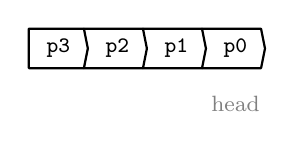
\begin{tikzpicture}

\coordinate (m1) at (-2.25,0);
\coordinate (m2) at (-1.5,0);
\coordinate (m3) at (-0.75,0);
\coordinate (m4) at (0,0);

\begin{scope}[scale=0.5, transform shape]
\pic at (m4) {queuenode={white}};
\pic at (m3) {queuenode={white}};
\pic at (m2) {queuenode={white}};
\pic at (m1) {queuenodetail={white}};
\end{scope}

\node at (m1) {\footnotesize\texttt{p3}};
\node at (m2) {\footnotesize\texttt{p2}};
\node at (m3) {\footnotesize\texttt{p1}};
\node at (m4) {\footnotesize\texttt{p0}};

\node[below of =m4, draw=white, yshift=3mm, width=1cm, smallgraytext] {head};

\end{tikzpicture}
\end{figure}

\end{frame}


\begin{frame}[fragile]
A \texttt{Queue} stores \texttt{QueueNode} objects and supports the following operations:\\~\\
\begin{itemize}


\item \highlight{\texttt{pop}} \\
\graytext{removes and returns the object with the maximum/minimum priority}\\[-1mm]
\begin{lstlisting}[style=mypython]
pop() -> Optional[QueueNode]
\end{lstlisting}


\item \highlight{\texttt{push}} \\
\graytext{inserts an object with priority \texttt{pri}}\\[-1mm]
\begin{lstlisting}[style=mypython]
push(pri: Integer, obj: Object) -> Optional[QueueNode]
\end{lstlisting}

\item \highlight{\texttt{peek}} \\
\graytext{returns the object with the maximum/minimum priority}\\[-1mm]
\begin{lstlisting}[style=mypython]
peek() -> Optional[QueueNode]
\end{lstlisting}

\end{itemize}
\end{frame}

\begin{frame}{Queues (via Binary Heaps)}
\begin{center}
\Large \highlight{\texttt{Queue}} \\[1mm] \normalsize \color{gray} (via Binary Heaps)
\end{center}
\end{frame}

\begin{frame}
\begin{thmbox}
A \highlight{\textbf{binary heap}} is a complete binary tree where each node's priority is greater than or equal to\footnote{This is called a max-heap. Alternatively, if each node’s priority is less than or equal to its children’s priorities, the structure is called a min-heap.} the priorities of its children, and
\begin{center}
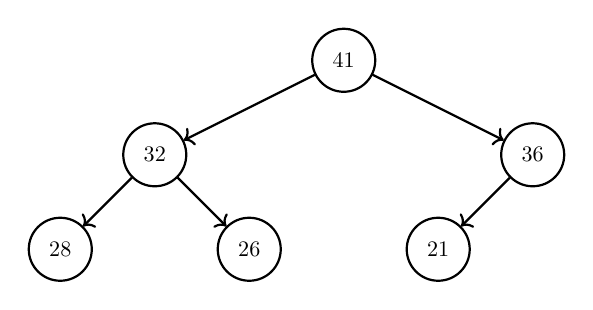
\begin{tikzpicture}[scale=0.8, transform shape]
\node[defaultnode] (n1) at (0,0)  { 41 };
\node[defaultnode] (n2) at (-3,-1.5)  { 32 };
\node[defaultnode] (n3) at (3,-1.5)  { 36 };
\node[defaultnode] (n4) at (-4.5,-3)  { 28 };
\node[defaultnode] (n5) at (1.5,-3)  { 21 };
\node[defaultnode] (n6) at (-1.5,-3)  { 26 };

\draw[thick, ->] (n1) -- (n2);
\draw[thick, ->] (n1) -- (n3);

\draw[thick, ->] (n2) -- (n4);
\draw[thick, ->] (n3) -- (n5);

\draw[thick, ->] (n2) -- (n6);

\end{tikzpicture}
\end{center}
This is called the \highlight{\textbf{heap-property}}.    
\end{thmbox}

\end{frame}

\begin{frame}[fragile]
\begin{thmboxtop}
\highlight{\texttt{Queue}} \\
\graytext{(via Binary Heaps)}
\begin{lstlisting}[style=mypython]
class QueueNode:
# attributes
    # the object of this node
    obj: Object

    # the priority of this node
    pri: Integer

    # the left child of this node
    left: Optional[QueueNode]

    # the right child of this node
    right: Optional[QueueNode]

    # the parent of this node
    pnt: Optional[QueueNode]
\end{lstlisting}
\end{thmboxtop}
\end{frame}

\begin{frame}[fragile]
\begin{thmboxbot}
\begin{lstlisting}[style=mypython]
class Queue:
# attributes
    # the head
    head: Optional[QueueNode]

# functions
    ...
\end{lstlisting}
\end{thmboxbot}
\end{frame}

\begin{frame}
\begin{center}
\highlight{\textbf{pop}} \\
\footnotesize\color{gray} \texttt{pop()}
\end{center}
\begin{center}

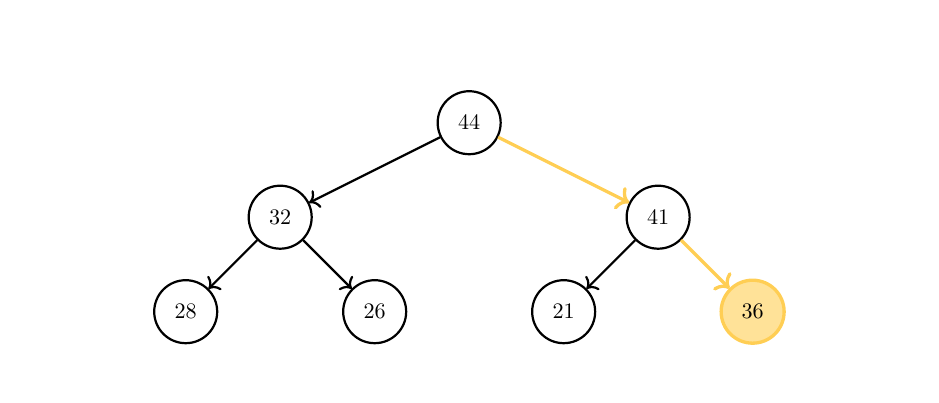
\begin{tikzpicture}[scale=0.8, transform shape]
\draw[white] (-7,-4) rectangle (7,1.5);
\node[defaultnode] (n1) at (0,0)  { 44 };
\node[defaultnode] (n2) at (-3,-1.5)  { 32 };
\node[defaultnode] (n3) at (3,-1.5)  { 41 };
\node[defaultnode] (n4) at (-4.5,-3)  { 28 };
\node[defaultnode] (n5) at (1.5,-3)  { 21 };
\node[newnode] (n7) at (4.5,-3)  { 36 };
\node[defaultnode] (n6) at (-1.5,-3)  { 26 };

\draw[thick, ->] (n1) -- (n2);
\draw[very thick, ->, myyellow] (n1) -- (n3);

\draw[thick, ->] (n2) -- (n4);
\draw[thick, ->] (n3) -- (n5);

\draw[thick, ->] (n2) -- (n6);
\draw[very thick, ->, myyellow] (n3) -- (n7);

\end{tikzpicture}
\end{center}
\begin{center}
\footnotesize\color{gray} find the last node
\end{center}    

\end{frame}


\begin{frame}
\begin{center}
\highlight{\textbf{pop}} \\
\footnotesize\color{gray} \texttt{pop()}
\end{center}
\begin{center}

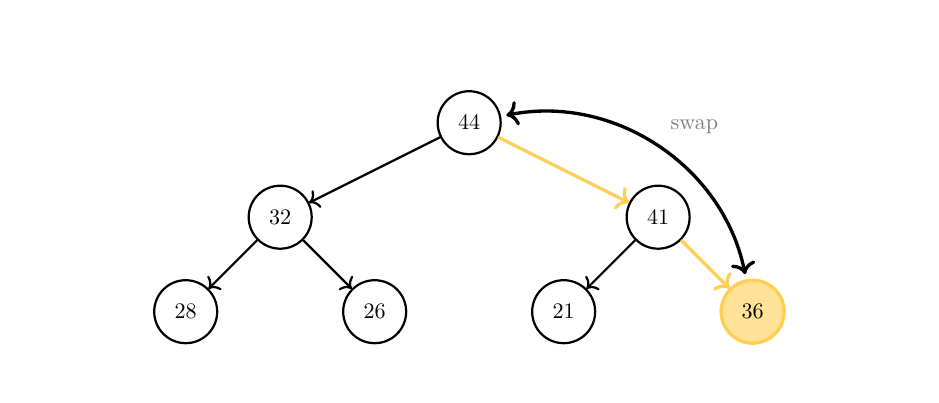
\begin{tikzpicture}[scale=0.8, transform shape]
\draw[white] (-7,-4) rectangle (7,1.5);
\node[defaultnode] (n1) at (0,0)  { 44 };
\node[defaultnode] (n2) at (-3,-1.5)  { 32 };
\node[defaultnode] (n3) at (3,-1.5)  { 41 };
\node[defaultnode] (n4) at (-4.5,-3)  { 28 };
\node[defaultnode] (n5) at (1.5,-3)  { 21 };
\node[newnode] (n7) at (4.5,-3)  { 36 };
\node[defaultnode] (n6) at (-1.5,-3)  { 26 };

\draw[thick, ->] (n1) -- (n2);
\draw[very thick, ->, myyellow] (n1) -- (n3);

\draw[thick, ->] (n2) -- (n4);
\draw[thick, ->] (n3) -- (n5);

\draw[thick, ->] (n2) -- (n6);
\draw[very thick, ->, myyellow] (n3) -- (n7);

\draw[very thick, <->, bend left, shorten >=2pt, shorten <=2pt] (n1) edge[bend left=45] node[above right=1mm] {\color{gray} swap} (n7);
\end{tikzpicture}
\end{center}
\begin{center}
\footnotesize\color{gray} swap the root with the last node in the heap
\end{center}    

\end{frame}

\begin{frame}
\begin{center}
\highlight{\textbf{pop}} \\
\footnotesize\color{gray} \texttt{pop()}
\end{center}
\begin{center}

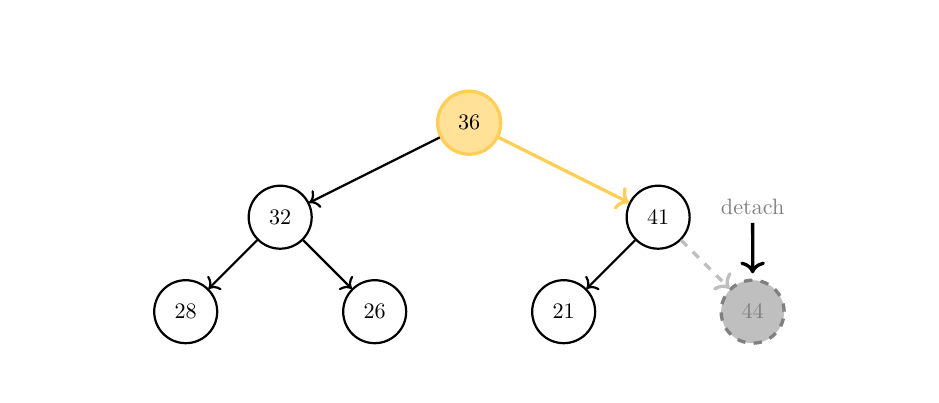
\begin{tikzpicture}[scale=0.8, transform shape]
\draw[white] (-7,-4) rectangle (7,1.5);
\node[newnode] (n1) at (0,0)  { 36 };
\node[defaultnode] (n2) at (-3,-1.5)  { 32 };
\node[defaultnode] (n3) at (3,-1.5)  { 41 };
\node[defaultnode] (n4) at (-4.5,-3)  { 28 };
\node[defaultnode] (n5) at (1.5,-3)  { 21 };
\node[deletenode] (n7) at (4.5,-3) { \color{gray} 44 };
\node[defaultnode] (n6) at (-1.5,-3)  { 26 };

\draw[thick, ->] (n1) -- (n2);
\draw[very thick, ->, myyellow] (n1) -- (n3);

\draw[thick, ->] (n2) -- (n4);
\draw[thick, ->] (n3) -- (n5);

\draw[thick, ->] (n2) -- (n6);
\draw[very thick, ->, dashed, lightgray] (n3) -- (n7);

\draw[very thick, shorten >=2pt, shorten <=2pt, <-]
(n7) edge node[above=4mm] {\color{gray} detach} ([yshift=1.5cm]n7);
\end{tikzpicture}
\end{center}
\begin{center}
\footnotesize\color{gray} detach the last node in the heap
\end{center}    
    
\end{frame}

\begin{frame}
\begin{center}
\highlight{\textbf{pop}} \\
\footnotesize\color{gray} \texttt{pop()}
\end{center}
\begin{center}

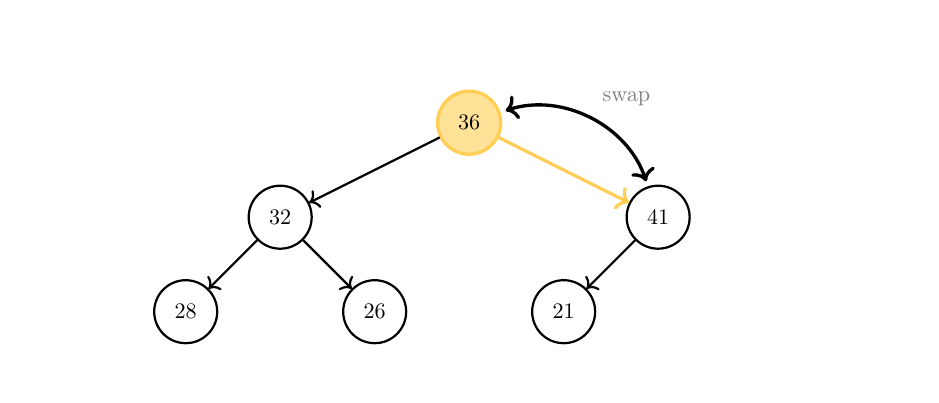
\begin{tikzpicture}[scale=0.8, transform shape]
\draw[white] (-7,-4) rectangle (7,1.5);
\node[newnode] (n1) at (0,0)  { 36 };
\node[defaultnode] (n2) at (-3,-1.5)  { 32 };
\node[defaultnode] (n3) at (3,-1.5)  { 41 };
\node[defaultnode] (n4) at (-4.5,-3)  { 28 };
\node[defaultnode] (n5) at (1.5,-3)  { 21 };
\node[opacity=0] (n7) at (4.5,-3)  { 44 };
\node[defaultnode] (n6) at (-1.5,-3)  { 26 };

\draw[thick, ->] (n1) -- (n2);
\draw[very thick, ->, myyellow] (n1) -- (n3);

\draw[thick, ->] (n2) -- (n4);
\draw[thick, ->] (n3) -- (n5);

\draw[thick, ->] (n2) -- (n6);
%\draw[thick, ->] (n3) -- (n7);

\draw[very thick, <->, bend left, shorten >=2pt, shorten <=2pt] (n1) edge[bend left=45] node[above right=1mm] {\color{gray} swap} (n3);
\end{tikzpicture}
\end{center}
\begin{center}
\footnotesize\color{gray} compare with larger child for the heap invariant and swap as needed
\end{center}    
\end{frame}

\begin{frame}
\begin{center}
\highlight{\textbf{pop}} \\
\footnotesize\color{gray} \texttt{pop()}
\end{center}
\begin{center}

\begin{tikzpicture}[scale=0.8, transform shape]
\draw[white] (-7,-4) rectangle (7,1.5);
\node[defaultnode] (n1) at (0,0)  { 41 };
\node[defaultnode] (n2) at (-3,-1.5)  { 32 };
\node[defaultnode] (n3) at (3,-1.5)  { 36 };
\node[defaultnode] (n4) at (-4.5,-3)  { 28 };
\node[defaultnode] (n5) at (1.5,-3)  { 21 };
\node[opacity=0] (n7) at (4.5,-3)  { 44 };
\node[defaultnode] (n6) at (-1.5,-3)  { 26 };

\draw[thick, ->] (n1) -- (n2);
\draw[thick, ->] (n1) -- (n3);

\draw[thick, ->] (n2) -- (n4);
\draw[thick, ->] (n3) -- (n5);

\draw[thick, ->] (n2) -- (n6);
%\draw[thick, ->] (n3) -- (n7);
\end{tikzpicture}
\end{center}
\begin{center}
\footnotesize\color{gray} \;
\end{center}    
\end{frame}

\begin{frame}
Because a complete binary tree is filled level-by-level, the last node can be found by following the bits of the heap’s size in binary (after the first), going left for 0 and right for 1.
\begin{center}
\Large $7$\color{lightgray}$_{10}$\color{black} $\;=$ \color{gray}$1$\color{myyellow}$11$\color{lightgray}$_2$
\end{center}

\begin{center}

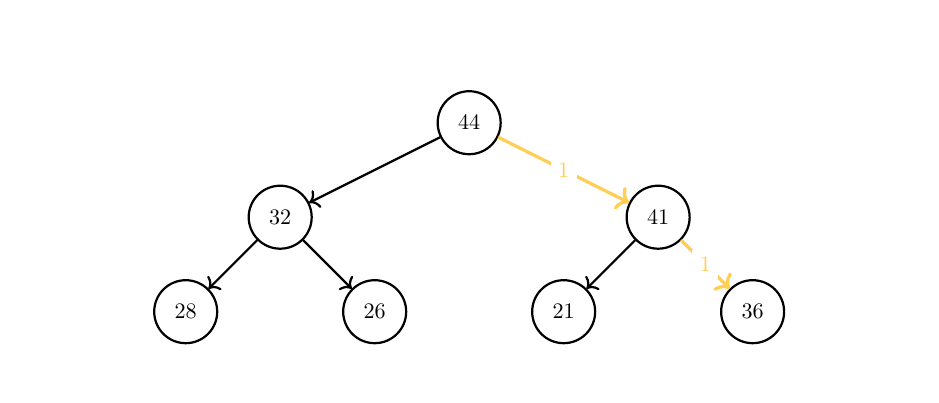
\begin{tikzpicture}[scale=0.8, transform shape]
\draw[white] (-7,-4) rectangle (7,1.5);
\node[defaultnode] (n1) at (0,0)  { 44 };
\node[defaultnode] (n2) at (-3,-1.5)  { 32 };
\node[defaultnode] (n3) at (3,-1.5)  { 41 };
\node[defaultnode] (n4) at (-4.5,-3)  { 28 };
\node[defaultnode] (n5) at (1.5,-3)  { 21 };
\node[defaultnode] (n7) at (4.5,-3)  { 36 };
\node[defaultnode] (n6) at (-1.5,-3)  { 26 };

\draw[thick, ->] (n1) -- (n2);
\draw[very thick, ->, myyellow] (n1) -- node[fill=white] {$1$} (n3);

\draw[thick, ->] (n2) -- (n4);
\draw[thick, ->] (n3) -- (n5);

\draw[thick, ->] (n2) -- (n6);
\draw[very thick, ->, myyellow] (n3) -- node[fill=white] {$1$} (n7);
\end{tikzpicture}
\end{center}
\begin{center}
\footnotesize\color{gray} this heap has a size of 7 which is 111 in binary
\end{center}
\end{frame}

\begin{frame}[fragile]
\begin{thmbox}
\begin{lstlisting}[style=mypython]
def pop(self: Queue) -> Optional[QueueNode]:
    if self.size == 0:
        return None
    max_val = self.root.pri
    
    if self.size == 1:
        root = self.root
        self.root = None
        self.size = 0
        return root
        
    last = self._detach()
    self._bubble_down(self.root)
    return last
\end{lstlisting}
\end{thmbox}
\end{frame}

\begin{frame}[fragile]
\begin{thmbox}
\begin{lstlisting}[style=mypython]
def _detach(self: Queue) -> Optional[QueueNode]:
    path = bin(self.size)[3:]  # skip '0b1'
    pnt = self.root
    for direction in path[:-1]:
        pnt = pnt.left if direction == '0' else pnt.right
    if path[-1] == '0':
        last = pnt.left
        pnt.left = None
    else:
        last = pnt.right
        pnt.right = None
    self.root.pri = last.pri
    self.root.obj = last.obj
    
    self.size -= 1
    return last

\end{lstlisting}
    
\end{thmbox}
\end{frame}


\begin{frame}[fragile]
\begin{thmbox}
\begin{lstlisting}[style=mypython]
def _bubble_down(self: QueueNode, node: QueueNode):
    while node:
        largest = node
        if node.left and node.left.pri > largest.pri:
            largest = node.left
        if node.right and node.right.pri > largest.pri:
            largest = node.right
        if largest == node:
            break
        # swap priorties
        node.pri, largest.pri = largest.pri, node.pri
        # swap objects
        node.obj, largest.obj = largest.obj, node.obj
        # continue with next node
        node = largest
\end{lstlisting}
\end{thmbox}
\end{frame}


\begin{frame}
\begin{center}
        \highlight{\textbf{push}} \\
        \footnotesize\color{gray} \texttt{push(44, obj)}
\end{center}
\begin{center}

\begin{tikzpicture}[scale=0.8, transform shape]
\draw[white] (-7,-4) rectangle (7,1.5);
    \node[defaultnode] (n1) at (0,0)  { 41 };
    \node[defaultnode] (n2) at (-3,-1.5)  { 32 };
    \node[defaultnode] (n3) at (3,-1.5)  { 36 };
    \node[defaultnode] (n4) at (-4.5,-3)  { 28 };
    \node[defaultnode] (n5) at (1.5,-3)  { 21 };
    \node[fill=white, opacity=0] (n7) at (4.5,-3)  { 44 };
    \node[defaultnode] (n6) at (-1.5,-3)  { 26 };

    \draw[thick, ->] (n1) -- (n2);
    \draw[thick, ->] (n1) -- (n3);

    \draw[thick, ->] (n2) -- (n4);
    \draw[thick, ->] (n3) -- (n5);

    \draw[thick, ->] (n2) -- (n6);
    
\end{tikzpicture}
\end{center}
\begin{center}
    \footnotesize\color{gray} \;
\end{center}    
    
\end{frame}

\begin{frame}
\begin{center}
\highlight{\textbf{push}} \\
\footnotesize\color{gray} \texttt{push(44, obj)}
\end{center}
\begin{center}

\begin{tikzpicture}[scale=0.8, transform shape]
\draw[white] (-7,-4) rectangle (7,1.5);
    \node[defaultnode] (n1) at (0,0)  { 41 };
    \node[defaultnode] (n2) at (-3,-1.5)  { 32 };
    \node[defaultnode] (n3) at (3,-1.5)  { 36 };
    \node[defaultnode] (n4) at (-4.5,-3)  { 28 };
    \node[defaultnode] (n5) at (1.5,-3)  { 21 };
    \node[fill=white, opacity=0] (n7) at (4.5,-3)  { 44 };
    \node[defaultnode] (n6) at (-1.5,-3)  { 26 };

    \draw[thick, ->] (n1) -- (n2);
    \draw[very thick, myyellow, ->] (n1) -- (n3);

    \draw[thick, ->] (n2) -- (n4);
    \draw[thick, ->] (n3) -- (n5);

    \draw[thick, ->] (n2) -- (n6);
    
\end{tikzpicture}
\end{center}
\begin{center}
\graytext{find the insertion point}
\end{center}    
    
\end{frame}

\begin{frame}
\begin{center}
        \highlight{\textbf{push}} \\
        \footnotesize\color{gray} \texttt{push(44, obj)}
\end{center}
\begin{center}
\normalsize\color{black}
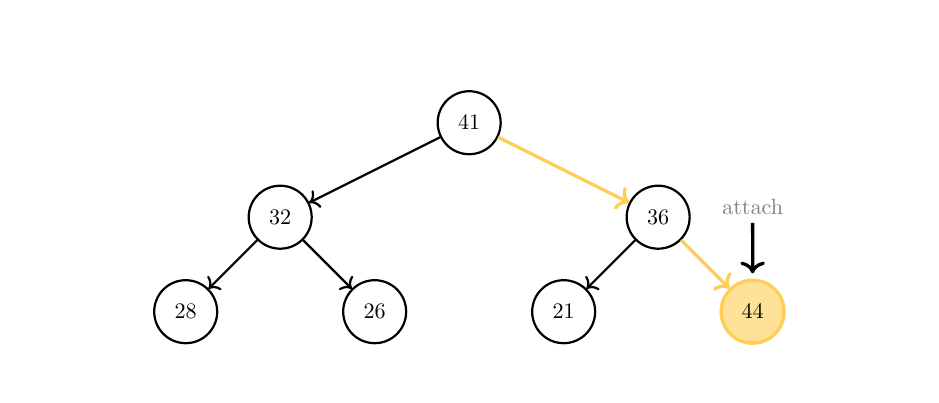
\begin{tikzpicture}[scale=0.8, transform shape]
\draw[white] (-7,-4) rectangle (7,1.5);
\node[defaultnode] (n1) at (0,0)  { 41 };
\node[defaultnode] (n2) at (-3,-1.5)  { 32 };
\node[defaultnode] (n3) at (3,-1.5)  { 36 };
\node[defaultnode] (n4) at (-4.5,-3)  { 28 };
\node[defaultnode] (n5) at (1.5,-3)  { 21 };
\node[newnode] (n7) at (4.5,-3)  { 44 };
\node[defaultnode] (n6) at (-1.5,-3)  { 26 };

\draw[thick, ->] (n1) -- (n2);
\draw[very thick, ->, myyellow] (n1) -- (n3);

\draw[thick, ->] (n2) -- (n4);
\draw[thick, ->] (n3) -- (n5);

\draw[thick, ->] (n2) -- (n6);
\draw[very thick, ->, myyellow] (n3) -- (n7);

\draw[very thick, shorten >=2pt, shorten <=2pt, <-]
(n7) edge node[above=4mm] {\color{gray} attach} ([yshift=1.5cm]n7);
\end{tikzpicture}
\end{center}
\begin{center}
\footnotesize\color{gray} insert the new node at the next available position
\end{center}    
    
\end{frame}

\begin{frame}
\begin{center}
        \highlight{\textbf{push}} \\
        \footnotesize\color{gray} \texttt{push(44, obj)}
\end{center}
\begin{center}
\normalsize\color{black}
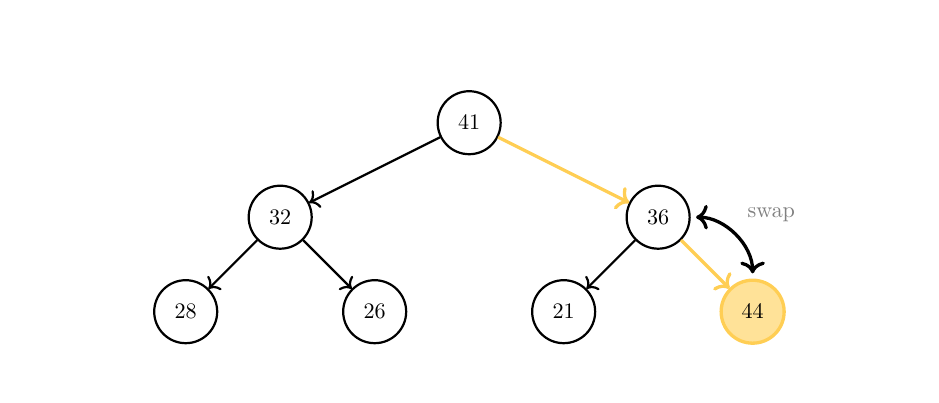
\begin{tikzpicture}[scale=0.8, transform shape]
\draw[white] (-7,-4) rectangle (7,1.5);
\node[defaultnode] (n1) at (0,0)  { 41 };
\node[defaultnode] (n2) at (-3,-1.5)  { 32 };
\node[defaultnode] (n3) at (3,-1.5)  { 36 };
\node[defaultnode] (n4) at (-4.5,-3)  { 28 };
\node[defaultnode] (n5) at (1.5,-3)  { 21 };
\node[newnode] (n7) at (4.5,-3)  { 44 };
\node[defaultnode] (n6) at (-1.5,-3)  { 26 };

\draw[thick, ->] (n1) -- (n2);
\draw[very thick, ->, myyellow] (n1) -- (n3);

\draw[thick, ->] (n2) -- (n4);
\draw[thick, ->] (n3) -- (n5);

\draw[thick, ->] (n2) -- (n6);
\draw[very thick, ->, myyellow] (n3) -- (n7);

\draw[very thick, <->, bend left, shorten >=2pt, shorten <=2pt] (n3) edge[bend left=45] node[above right=1mm] {\color{gray} swap} (n7);
\end{tikzpicture}
\end{center}
\begin{center}
\footnotesize\color{gray} compare with parent for the heap invariant and swap as needed
\end{center}    
    
\end{frame}


\begin{frame}
\begin{center}
\highlight{\textbf{push}} \\
\footnotesize\color{gray} \texttt{push(44, obj)}
\end{center}
\begin{center}
\normalsize\color{black}
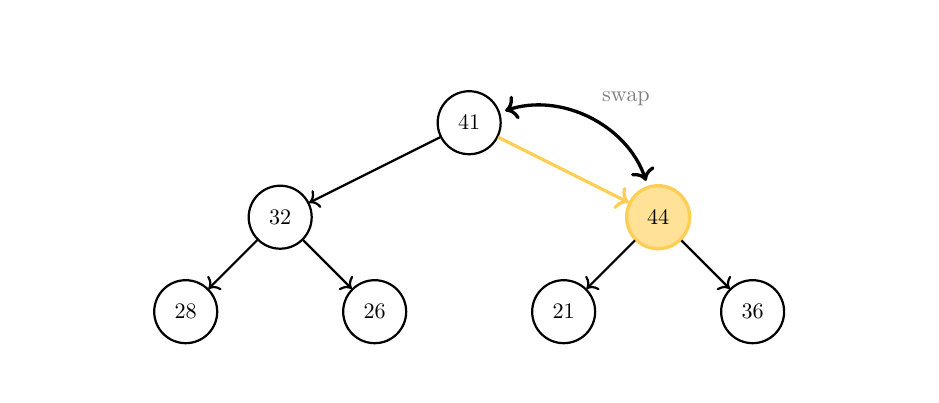
\begin{tikzpicture}[scale=0.8, transform shape]
\draw[white] (-7,-4) rectangle (7,1.5);
\node[defaultnode] (n1) at (0,0)  { 41 };
\node[defaultnode] (n2) at (-3,-1.5)  { 32 };
\node[newnode] (n3) at (3,-1.5)  { 44 };
\node[defaultnode] (n4) at (-4.5,-3)  { 28 };
\node[defaultnode] (n5) at (1.5,-3)  { 21 };
\node[defaultnode] (n7) at (4.5,-3)  { 36 };
\node[defaultnode] (n6) at (-1.5,-3)  { 26 };

\draw[thick, ->] (n1) -- (n2);
\draw[very thick, ->, myyellow] (n1) -- (n3);

\draw[thick, ->] (n2) -- (n4);
\draw[thick, ->] (n3) -- (n5);

\draw[thick, ->] (n2) -- (n6);
\draw[thick, ->] (n3) -- (n7);

\draw[very thick, <->, bend left, shorten >=2pt, shorten <=2pt] (n1) edge[bend left=45] node[above right=1mm] {\color{gray} swap} (n3);
\end{tikzpicture}
\end{center}
\begin{center}
\footnotesize\color{gray} compare with parent for the heap invariant and swap as needed
\end{center}    
\end{frame}

\begin{frame}
\begin{center}
\highlight{\textbf{push}} \\
\footnotesize\color{gray} \texttt{push(44, obj)}
\end{center}
\begin{center}
\normalsize\color{black}
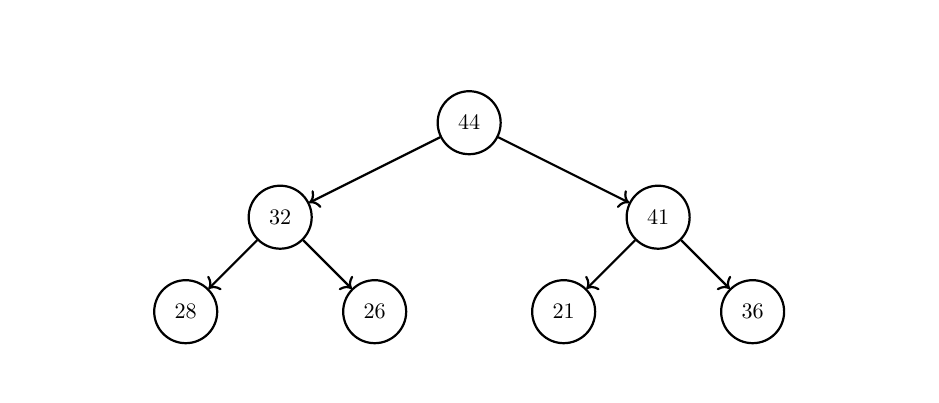
\begin{tikzpicture}[scale=0.8, transform shape]
\draw[white] (-7,-4) rectangle (7,1.5);
\node[defaultnode] (n1) at (0,0)  { 44 };
\node[defaultnode] (n2) at (-3,-1.5)  { 32 };
\node[defaultnode] (n3) at (3,-1.5)  { 41 };
\node[defaultnode] (n4) at (-4.5,-3)  { 28 };
\node[defaultnode] (n5) at (1.5,-3)  { 21 };
\node[defaultnode] (n7) at (4.5,-3)  { 36 };
\node[defaultnode] (n6) at (-1.5,-3)  { 26 };

\draw[thick, ->] (n1) -- (n2);
\draw[thick, ->] (n1) -- (n3);

\draw[thick, ->] (n2) -- (n4);
\draw[thick, ->] (n3) -- (n5);

\draw[thick, ->] (n2) -- (n6);
\draw[thick, ->] (n3) -- (n7);
\end{tikzpicture}
\end{center}
\begin{center}
\footnotesize\color{gray} \;
\end{center}    
\end{frame}

\begin{frame}
Because a complete binary tree is filled level-by-level, the next insertion point can be found by following the bits of the heap’s size in binary plus one (after the first), going left for 0 and right for 1.
\begin{center}
\Large $(6+1)$\color{lightgray}$_{10}$\color{black} $\;=$ \color{gray}$1$\color{myyellow}$11$\color{lightgray}$_2$
\end{center}

\begin{center}

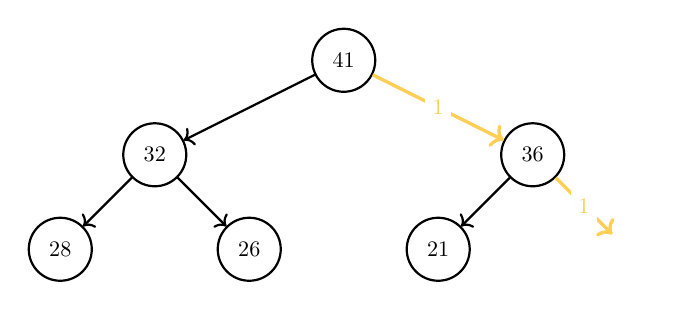
\begin{tikzpicture}[scale=0.8, transform shape]
    \node[defaultnode] (n1) at (0,0)  { 41 };
    \node[defaultnode] (n2) at (-3,-1.5)  { 32 };
    \node[defaultnode] (n3) at (3,-1.5)  { 36 };
    \node[defaultnode] (n4) at (-4.5,-3)  { 28 };
    \node[defaultnode] (n5) at (1.5,-3)  { 21 };
    \node[fill=white, opacity=0] (n7) at (4.5,-3)  { 44 };
    \node[defaultnode] (n6) at (-1.5,-3)  { 26 };

    \draw[thick, ->] (n1) -- (n2);
    \draw[very thick, ->, myyellow] (n1) --  node[fill=white] {$1$} (n3);

    \draw[thick, ->] (n2) -- (n4);
    \draw[thick, ->] (n3) -- (n5);

    \draw[thick, ->] (n2) -- (n6);
    \draw[very thick, ->, myyellow] (n3) -- node[fill=white] {$1$} (n7);
\end{tikzpicture}
\end{center}
\begin{center}
    \footnotesize\color{gray} this heap has a size of 6 which is 110 in binary
\end{center}
\end{frame}

\begin{frame}[fragile]
\begin{thmboxtop}
\begin{lstlisting}[style=mypython]
def push(self: Queue, obj: Object, pri: Integer) -> Optional[QueueNode]:
    new_node = QueueNode(obj, pri)
    self.size += 1
    
    if self.size == 1:
        self.root = new_node
        return
        
    self._attach(new_node)
    self._bubble_up(new_node)
    return new_node
\end{lstlisting}
\end{thmboxtop}
\end{frame}

\begin{frame}[fragile]
\begin{thmboxside}
\begin{lstlisting}[style=mypython]
    def _attach(self: Queue, node: QueueNode) -> Optional[QueueNode]:
        size = self.size
        pnt = self.root
        
        while size > 0:
            if size & 1 == 0     
        
        for direction in path[:-1]:
            pnt = pnt.left if direction == '0' else pnt.right
        if path[-1] == '0':
            pnt.left = node
        else:
            pnt.right = node
        node.pnt = pnt
        return node
\end{lstlisting}
\end{thmboxside}
\end{frame}



\begin{frame}[fragile]
\begin{thmboxbot}
\begin{lstlisting}[style=mypython]
    def _bubble_up(self, node: QueueNode):
        while node and node.pnt:
            largest = node.pnt
            if node.pri > largest.pri:
                # swap priorities
                node.pri, largest.pri = largest.pri, node.pri
                # swap objects
                node.obj, largest.obj = largest.obj, node.obj
                # continue upward
                node = largest
            else:
                break
\end{lstlisting}
\end{thmboxbot}
\end{frame}

\begin{frame}
\begin{center}
\highlight{\textbf{pop}} \\
\footnotesize\color{gray} \texttt{pop()}
\end{center}
\begin{center}

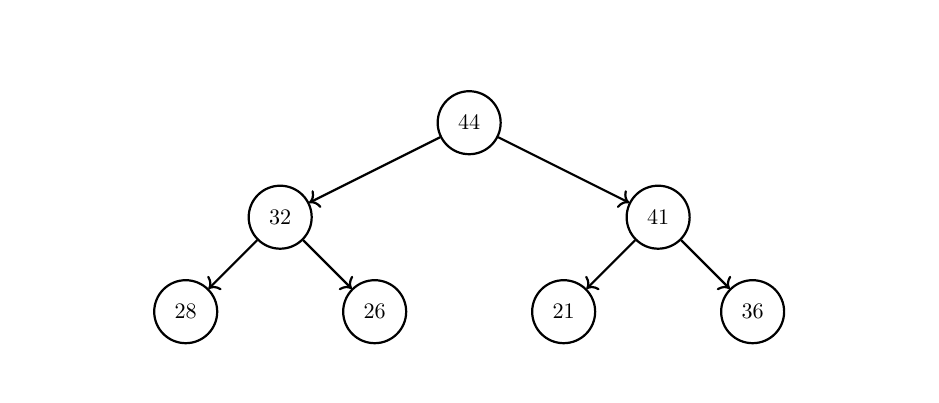
\begin{tikzpicture}[scale=0.8, transform shape]
\draw[white] (-7,-4) rectangle (7,1.5);
\node[defaultnode] (n1) at (0,0)  { 44 };
\node[defaultnode] (n2) at (-3,-1.5)  { 32 };
\node[defaultnode] (n3) at (3,-1.5)  { 41 };
\node[defaultnode] (n4) at (-4.5,-3)  { 28 };
\node[defaultnode] (n5) at (1.5,-3)  { 21 };
\node[defaultnode] (n7) at (4.5,-3)  { 36 };
\node[defaultnode] (n6) at (-1.5,-3)  { 26 };

\draw[thick, ->] (n1) -- (n2);
\draw[thick, ->] (n1) -- (n3);

\draw[thick, ->] (n2) -- (n4);
\draw[thick, ->] (n3) -- (n5);

\draw[thick, ->] (n2) -- (n6);
\draw[thick, ->] (n3) -- (n7);

\end{tikzpicture}
\end{center}
\begin{center}
\footnotesize\color{gray} \;
\end{center}    

\end{frame}


\begin{frame}
Properties of the \texttt{Queue} data-structure (via Binary Heaps):
\begin{table}
\begin{tabular}{@{} r | l @{} }
\highlight{\textbf{Property}} & \\[1mm]\hline
\multirow{1}{*}{Time Complexity} & \\
\color{gray}\footnotesize\texttt{insert} & \color{gray}\footnotesize $O(\log(N))$\\[1mm]
\color{gray}\footnotesize\texttt{peak} & \color{gray}\footnotesize $O(1)$ \\[1mm]
\color{gray}\footnotesize\texttt{pop} & \color{gray}\footnotesize $O(\log(N))$\\[1mm]
Space Complexity & $O(N)$
\end{tabular}
\end{table}
\begin{center}
\footnotesize\color{gray} properties of the \texttt{Queue} data-structure (via Binary Heaps)
\end{center}
\renewcommand\thefootnote{}\footnotetext{\color{gray} Assumptions: $N = $ \texttt{Queue.size}}
\end{frame}

\begin{frame}
Heaps can be implemented using only arrays with level-order 0-indexing.
\begin{table}
\begin{tabular}{@{} c | c | c | c @{} }
\textbf{node} & \textbf{parent} & \textbf{left child} & \textbf{right child} \\[1mm]\hline
$i$ & $\lfloor (i - 1) / 2 \rfloor$ & $2i + 1$ & $2i + 2$ \\[1mm]
\end{tabular}
\end{table}


\begin{center}

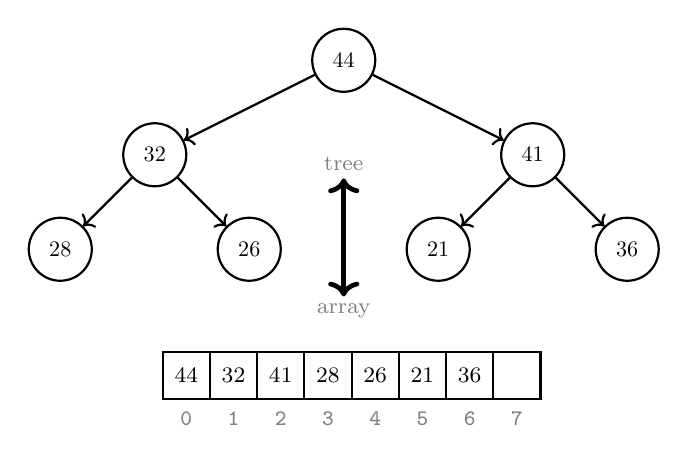
\begin{tikzpicture}
\begin{scope}[scale=0.8, transform shape]
\node[defaultnode] (n1) at (0,0)  { 44 };
\node[defaultnode] (n2) at (-3,-1.5)  { 32 };
\node[defaultnode] (n3) at (3,-1.5)  { 41 };
\node[defaultnode] (n4) at (-4.5,-3)  { 28 };
\node[defaultnode] (n5) at (1.5,-3)  { 21 };
\node[defaultnode] (n7) at (4.5,-3)  { 36 };
\node[defaultnode] (n6) at (-1.5,-3)  { 26 };

\draw[thick, ->] (n1) -- (n2);
\draw[thick, ->] (n1) -- (n3);

\draw[thick, ->] (n2) -- (n4);
\draw[thick, ->] (n3) -- (n5);

\draw[thick, ->] (n2) -- (n6);
\draw[thick, ->] (n3) -- (n7);
\end{scope}

\draw[line width=0.6mm, <->] 
  (0,-1.5) -- 
  node[above=7mm] {\footnotesize\color{gray} tree}
  node[below=7mm] {\footnotesize\color{gray} array}
  (0,-3);


\begin{scope}[yshift = -4cm, xshift=-2cm, every node/.style={shape=rectangle,
                                        draw=black,
                                        thick,
                                        fill=white,
                                        minimum size=6mm,
                                        inner sep=0pt}]
\node[draw=white, smallgraytext] (l1) at (0,-0.55) {\texttt{0}};
\node[draw=white, smallgraytext] (l2) at (0.6,-0.55) {\texttt{1}};
\node[draw=white, smallgraytext] (l3) at (1.2,-0.55) {\texttt{2}};
\node[draw=white, smallgraytext] (l4) at (1.8,-0.55) {\texttt{3}};
\node[draw=white, smallgraytext] (l5) at (2.4,-0.55) {\texttt{4}};
\node[draw=white, smallgraytext] (l6) at (3.0,-0.55) {\texttt{5}};
\node[draw=white, smallgraytext] (l7) at (3.6,-0.55) {\texttt{6}};
\node[draw=white, smallgraytext] (l8) at (4.2,-0.55) {\texttt{7}};

\node (m1) at (0,0) {\footnotesize 44};
\node (m2) at (0.6,0) {\footnotesize 32};
\node (m3) at (1.2,0) {\footnotesize 41};
\node (m4) at (1.8,0) {\footnotesize 28};
\node (m5) at (2.4,0) {\footnotesize 26};
\node (m6) at (3.0,0) {\footnotesize 21};
\node (m7) at (3.6,0) {\footnotesize 36};
\node (m8) at (4.2,0) {\footnotesize  };
\end{scope}
\end{tikzpicture}
\end{center}
\end{frame}


\begin{frame}{Appendix (proofs)}
\begin{center}
\Large \highlight{\textbf{appendix}} \\[1mm]
\normalsize \color{gray} (proofs)
\end{center}
\end{frame}


\begin{frame}
\begin{thmbox}
The time complexity of \texttt{pop} for \texttt{Queue} (via Binary Heaps) is $O(\log N)$, where $N = $ \texttt{Queue.size}.
\end{thmbox}
\begin{thmboxtop}
\highlightc{lightgray}{\textbf{finding the last node}}: \hfill $O(\log N)$ \\[1mm]
\footnotesize\color{gray}
Since the heap is a complete binary tree, its height is at most $\cei{\log(N)}$. Thus, we traverse at most $\ceil{\log(N)}$ nodes to the last node. \\[-3mm] 
\begin{center}
\normalsize\color{black}
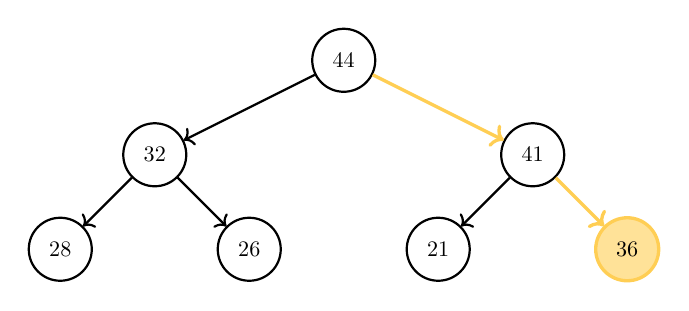
\begin{tikzpicture}[scale=0.8, transform shape]
\node[defaultnode] (n1) at (0,0)  { 44 };
\node[defaultnode] (n2) at (-3,-1.5)  { 32 };
\node[defaultnode] (n3) at (3,-1.5)  { 41 };
\node[defaultnode] (n4) at (-4.5,-3)  { 28 };
\node[defaultnode] (n5) at (1.5,-3)  { 21 };
\node[newnode] (n7) at (4.5,-3)  { 36 };
\node[defaultnode] (n6) at (-1.5,-3)  { 26 };

\draw[thick, ->] (n1) -- (n2);
\draw[very thick, ->, myyellow] (n1) -- (n3);

\draw[thick, ->] (n2) -- (n4);
\draw[thick, ->] (n3) -- (n5);

\draw[thick, ->] (n2) -- (n6);
\draw[very thick, ->, myyellow] (n3) -- (n7);
\end{tikzpicture}
\end{center}
\begin{center}
\footnotesize\color{gray} \texttt{pop()}
\end{center}
\vspace{-5mm}
\hfill \graytext{\textit{(cont'd...)}}
\end{thmboxtop}
\end{frame}

\begin{frame}
\begin{thmboxside}
\highlightc{lightgray}{\textbf{swapping the root and last node}}: \hfill $O(1)$ \\[1mm]
\footnotesize\color{gray}
We swap the root with the last node, which takes $O(1)$ time. \\
\begin{center}
\normalsize\color{black}
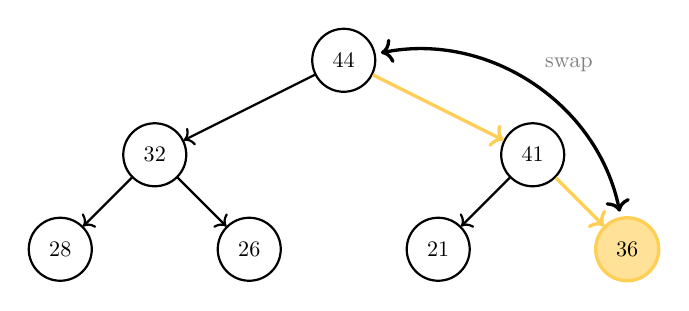
\begin{tikzpicture}[scale=0.8, transform shape]
\node[defaultnode] (n1) at (0,0)  { 44 };
\node[defaultnode] (n2) at (-3,-1.5)  { 32 };
\node[defaultnode] (n3) at (3,-1.5)  { 41 };
\node[defaultnode] (n4) at (-4.5,-3)  { 28 };
\node[defaultnode] (n5) at (1.5,-3)  { 21 };
\node[newnode] (n7) at (4.5,-3)  { 36 };
\node[defaultnode] (n6) at (-1.5,-3)  { 26 };

\draw[thick, ->] (n1) -- (n2);
\draw[very thick, ->, myyellow] (n1) -- (n3);

\draw[thick, ->] (n2) -- (n4);
\draw[thick, ->] (n3) -- (n5);

\draw[thick, ->] (n2) -- (n6);
\draw[very thick, ->, myyellow] (n3) -- (n7);

\draw[very thick, <->, bend left, shorten >=2pt, shorten <=2pt] (n1) edge[bend left=45] node[above right=1mm] {\color{gray} swap} (n7);
\end{tikzpicture}
\end{center}
\begin{center}
\footnotesize\color{gray} \texttt{pop()}
\end{center}
\end{thmboxside}
\end{frame}

\begin{frame}
\begin{thmboxside}
\highlightc{lightgray}{\textbf{removing the last node}}: \hfill $O(1)$ \\[1mm]
\footnotesize\color{gray}
The last node is detached from the tree, which takes $O(1)$ time.\\
\begin{center}
\normalsize\color{black}
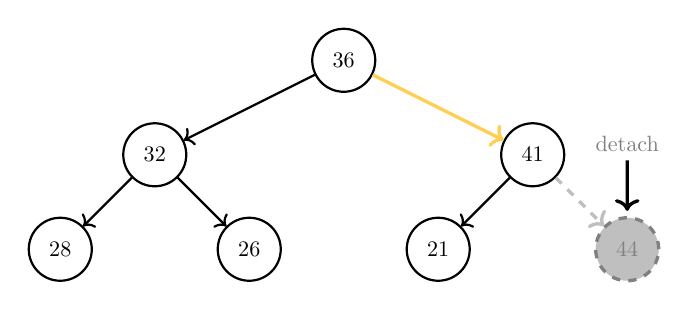
\begin{tikzpicture}[scale=0.8, transform shape]
\node[defaultnode] (n1) at (0,0)  { 36 };
\node[defaultnode] (n2) at (-3,-1.5)  { 32 };
\node[defaultnode] (n3) at (3,-1.5)  { 41 };
\node[defaultnode] (n4) at (-4.5,-3)  { 28 };
\node[defaultnode] (n5) at (1.5,-3)  { 21 };
\node[deletenode] (n7) at (4.5,-3) { \color{gray} 44 };
\node[defaultnode] (n6) at (-1.5,-3)  { 26 };

\draw[thick, ->] (n1) -- (n2);
\draw[very thick, ->, myyellow] (n1) -- (n3);

\draw[thick, ->] (n2) -- (n4);
\draw[thick, ->] (n3) -- (n5);

\draw[thick, ->] (n2) -- (n6);
\draw[very thick, ->, dashed, lightgray] (n3) -- (n7);

\draw[very thick, shorten >=2pt, shorten <=2pt, <-]
  (n7) edge node[above=4mm] {\color{gray} detach} ([yshift=1.5cm]n7);
\end{tikzpicture}
\end{center}
\end{thmboxside}
\end{frame}


\begin{frame}
\begin{thmboxbot}
\normalsize\color{black}
\highlightc{lightgray}{\textbf{restoring the heap property}}: \hfill $O(\log N)$ \\[1mm]
\footnotesize\color{gray}
We may need to bubble the root down by comparing it to its children and swapping if needed. Each swap takes $O(1)$ time, and there can be at most $\ceil{\log(N)}$ swaps before there are no more children.
\begin{center}
\normalsize\color{black}
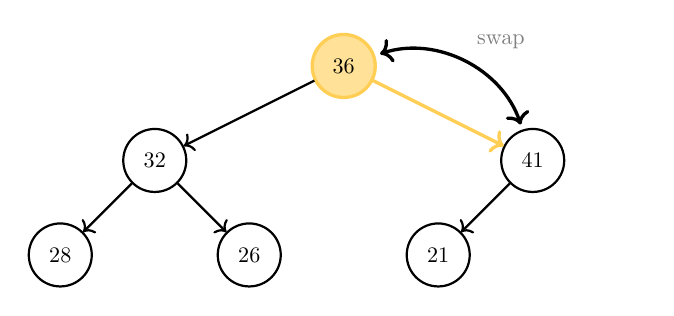
\begin{tikzpicture}[scale=0.8, transform shape]
\node[newnode] (n1) at (0,0)  { 36 };
\node[defaultnode] (n2) at (-3,-1.5)  { 32 };
\node[defaultnode] (n3) at (3,-1.5)  { 41 };
\node[defaultnode] (n4) at (-4.5,-3)  { 28 };
\node[defaultnode] (n5) at (1.5,-3)  { 21 };
\node[fill=white, opacity=0] (n7) at (4.5,-3)  { 44 };
\node[defaultnode] (n6) at (-1.5,-3)  { 26 };

\draw[thick, ->] (n1) -- (n2);
\draw[very thick, ->, myyellow] (n1) -- (n3);

\draw[thick, ->] (n2) -- (n4);
\draw[thick, ->] (n3) -- (n5);

\draw[thick, ->] (n2) -- (n6);
\draw[very thick, ->, opacity=0] (n3) -- (n7);

\draw[very thick, <->, bend left, shorten >=2pt, shorten <=2pt] (n1) edge[bend left=45] node[above right=1mm] {\color{gray} swap} (n3);
\end{tikzpicture}
\end{center}
\begin{center}
\footnotesize\color{gray} \texttt{pop()}
\end{center}
\end{thmboxbot}    
\end{frame}


\begin{frame}
\begin{thmbox}
The time complexity of \texttt{push} for \texttt{Queue} (via Binary Heaps) is $O(\log N)$, where  $N = $ \texttt{Queue.size}.
\end{thmbox}
\begin{thmboxtop}
\highlightc{lightgray}{\textbf{finding the insertion point}}: \hfill $O(\log N)$ \\[1mm]
\footnotesize\color{gray}
Since the heap is a complete binary tree, its height is at most $\ceil{\log(N)}$:\vspace{-1mm}
\begin{itemize}
\footnotesize\color{gray}
    \item when the tree has a height of $l$, it can hold $2^0 + \dots + 2^l = 2^{l+1}-1$ nodes\vspace{-1mm}
    \item assuming $2^{l+1}-1 = N$, it follows that $l = \log(N+1)-1 \leq \ceil{\log(N)}$
\end{itemize}
\vspace{-1mm}
Thus, we traverse at most $\ceil{\log(N)}$ nodes to the insertion point. \\[-3mm] 
\begin{center}
\normalsize\color{black}
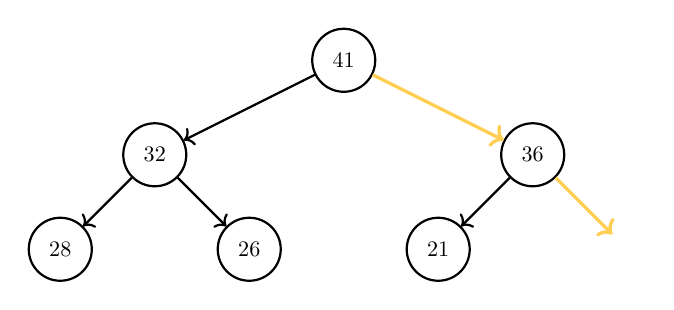
\begin{tikzpicture}[scale=0.8, transform shape]
\node[defaultnode] (n1) at (0,0)  { 41 };
\node[defaultnode] (n2) at (-3,-1.5)  { 32 };
\node[defaultnode] (n3) at (3,-1.5)  { 36 };
\node[defaultnode] (n4) at (-4.5,-3)  { 28 };
\node[defaultnode] (n5) at (1.5,-3)  { 21 };
\node[fill=white, opacity=0] (n7) at (4.5,-3)  { 44 };
\node[defaultnode] (n6) at (-1.5,-3)  { 26 };

\draw[thick, ->] (n1) -- (n2);
\draw[very thick, ->, myyellow] (n1) -- (n3);

\draw[thick, ->] (n2) -- (n4);
\draw[thick, ->] (n3) -- (n5);

\draw[thick, ->] (n2) -- (n6);
\draw[very thick, ->, myyellow] (n3) -- (n7);
\end{tikzpicture}
\end{center}
\begin{center}
\footnotesize\color{gray} \texttt{push(44, obj)}
\end{center}
\end{thmboxtop}
\end{frame}

\begin{frame}
\begin{thmboxside}
\highlightc{lightgray}{\textbf{inserting the new node}}: \hfill $O(1)$ \\[1mm]
\footnotesize\color{gray}
Attaching the new node to its parent takes $O(1)$ time.
\begin{center}
\normalsize\color{black}
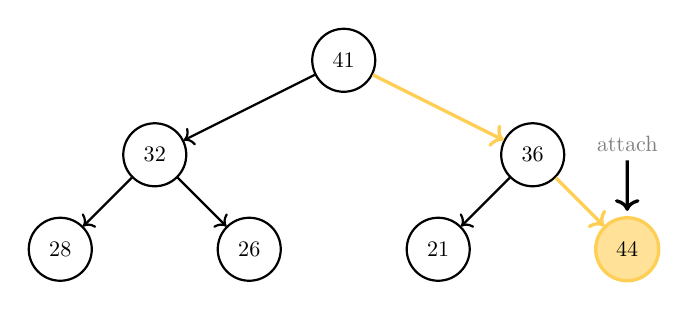
\begin{tikzpicture}[scale=0.8, transform shape]
\node[defaultnode] (n1) at (0,0)  { 41 };
\node[defaultnode] (n2) at (-3,-1.5)  { 32 };
\node[defaultnode] (n3) at (3,-1.5)  { 36 };
\node[defaultnode] (n4) at (-4.5,-3)  { 28 };
\node[defaultnode] (n5) at (1.5,-3)  { 21 };
\node[newnode] (n7) at (4.5,-3)  { 44 };
\node[defaultnode] (n6) at (-1.5,-3)  { 26 };

\draw[thick, ->] (n1) -- (n2);
\draw[very thick, ->, myyellow] (n1) -- (n3);

\draw[thick, ->] (n2) -- (n4);
\draw[thick, ->] (n3) -- (n5);

\draw[thick, ->] (n2) -- (n6);
\draw[very thick, ->, myyellow] (n3) -- (n7);

\draw[very thick, shorten >=2pt, shorten <=2pt, <-]
(n7) edge node[above=4mm] {\color{gray} attach} ([yshift=1.5cm]n7);
\end{tikzpicture}
\end{center}
\begin{center}
\footnotesize\color{gray} \texttt{push(44, obj)}
\end{center}
\end{thmboxside}
\end{frame}

\begin{frame}
\begin{thmboxbot}
\highlightc{lightgray}{\textbf{restoring the heap property}}: \hfill $O(\log N)$ \\[1mm]
\footnotesize\color{gray}
We may need to bubble the node up by comparing it to its parent and swapping if needed. Each swap takes $O(1)$ time, and there can be at most $\ceil{\log(N)}$ swaps on the path back to the root.
\begin{center}
\normalsize\color{black}
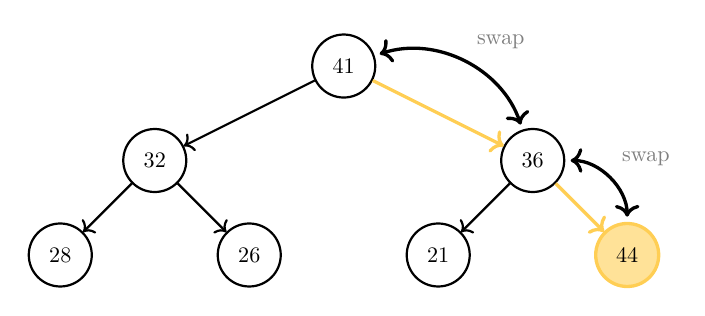
\begin{tikzpicture}[scale=0.8, transform shape]
\node[defaultnode] (n1) at (0,0)  { 41 };
\node[defaultnode] (n2) at (-3,-1.5)  { 32 };
\node[defaultnode] (n3) at (3,-1.5)  { 36 };
\node[defaultnode] (n4) at (-4.5,-3)  { 28 };
\node[defaultnode] (n5) at (1.5,-3)  { 21 };
\node[newnode] (n7) at (4.5,-3)  { 44 };
\node[defaultnode] (n6) at (-1.5,-3)  { 26 };

\draw[thick, ->] (n1) -- (n2);
\draw[very thick, ->, myyellow] (n1) -- (n3);

\draw[thick, ->] (n2) -- (n4);
\draw[thick, ->] (n3) -- (n5);

\draw[thick, ->] (n2) -- (n6);
\draw[very thick, ->, myyellow] (n3) -- (n7);

\draw[very thick, <->, bend left, shorten >=2pt, shorten <=2pt] (n3) edge[bend left=45] node[above right=1mm] {\color{gray} swap} (n7);
\draw[very thick, <->, bend left, shorten >=2pt, shorten <=2pt] (n1) edge[bend left=45] node[above right=1mm] {\color{gray} swap} (n3);
\end{tikzpicture}
\end{center}
\begin{center}
\footnotesize\color{gray} \texttt{push(44, obj)}
\end{center}
\end{thmboxbot}
\end{frame}

\begin{frame}
\begin{thmbox}
The time complexity of \texttt{peak} for \texttt{Queue} (via Binary Heaps) is $O(1)$.
\end{thmbox}
\begin{proofbox}
\highlightc{lightgray}{\textbf{accessing the root}}: \hfill $O(1)$ \\[1mm]
\footnotesize\color{gray}
In a binary heap, the highest (or lowest) priority element is always stored at the root. Accessing the root takes $O(1)$ time.
\end{proofbox}
\end{frame}

\end{document}